\appendix
\chapter{Sec'tiuni relevante din cod}

\begin{verbatim}
 /** Maps are easy to use in Scala. */
object Maps {
  val colors = Map("red" -> 0xFF0000,
                   "turquoise" -> 0x00FFFF,
                   "black" -> 0x000000,
                   "orange" -> 0xFF8040,
                   "brown" -> 0x804000)
  def main(args: Array[String]) {
    for (name <- args) println(
      colors.get(name) match {
        case Some(code) =>
          name + " has code: " + code
        case None =>
          "Unknown color: " + name
      }
    )
  }
}
\end{verbatim}

\chapter{Alte informa'tii relevante (demonstra'tii etc.)}

\textcolor{green}{LISTA DE INTREBARI PERMISE}

\chapter{Lucr'ari publicate (dac'a exist'a)}

Agentul explicabil pentru 'inv'a'tare automat'a descris 'in aceast'a lucrare a fost prezentat 'si 'in articolul "Towards Explainable Machine Learning Using  Natural Language Processing and Ontologies". Articolul este trimis la "IEEE 15th International Conference on
Intelligent Computer Communication and Processing (ICCP 2019)" 'si se afl'a in curs de verificare. Cu o variant'a restr\ia ns'a a acestuia am participat la "Conferin'ta 'Stiin'tific'a a Studen'tilor Sec'tiilor de Calculatoare 2019".
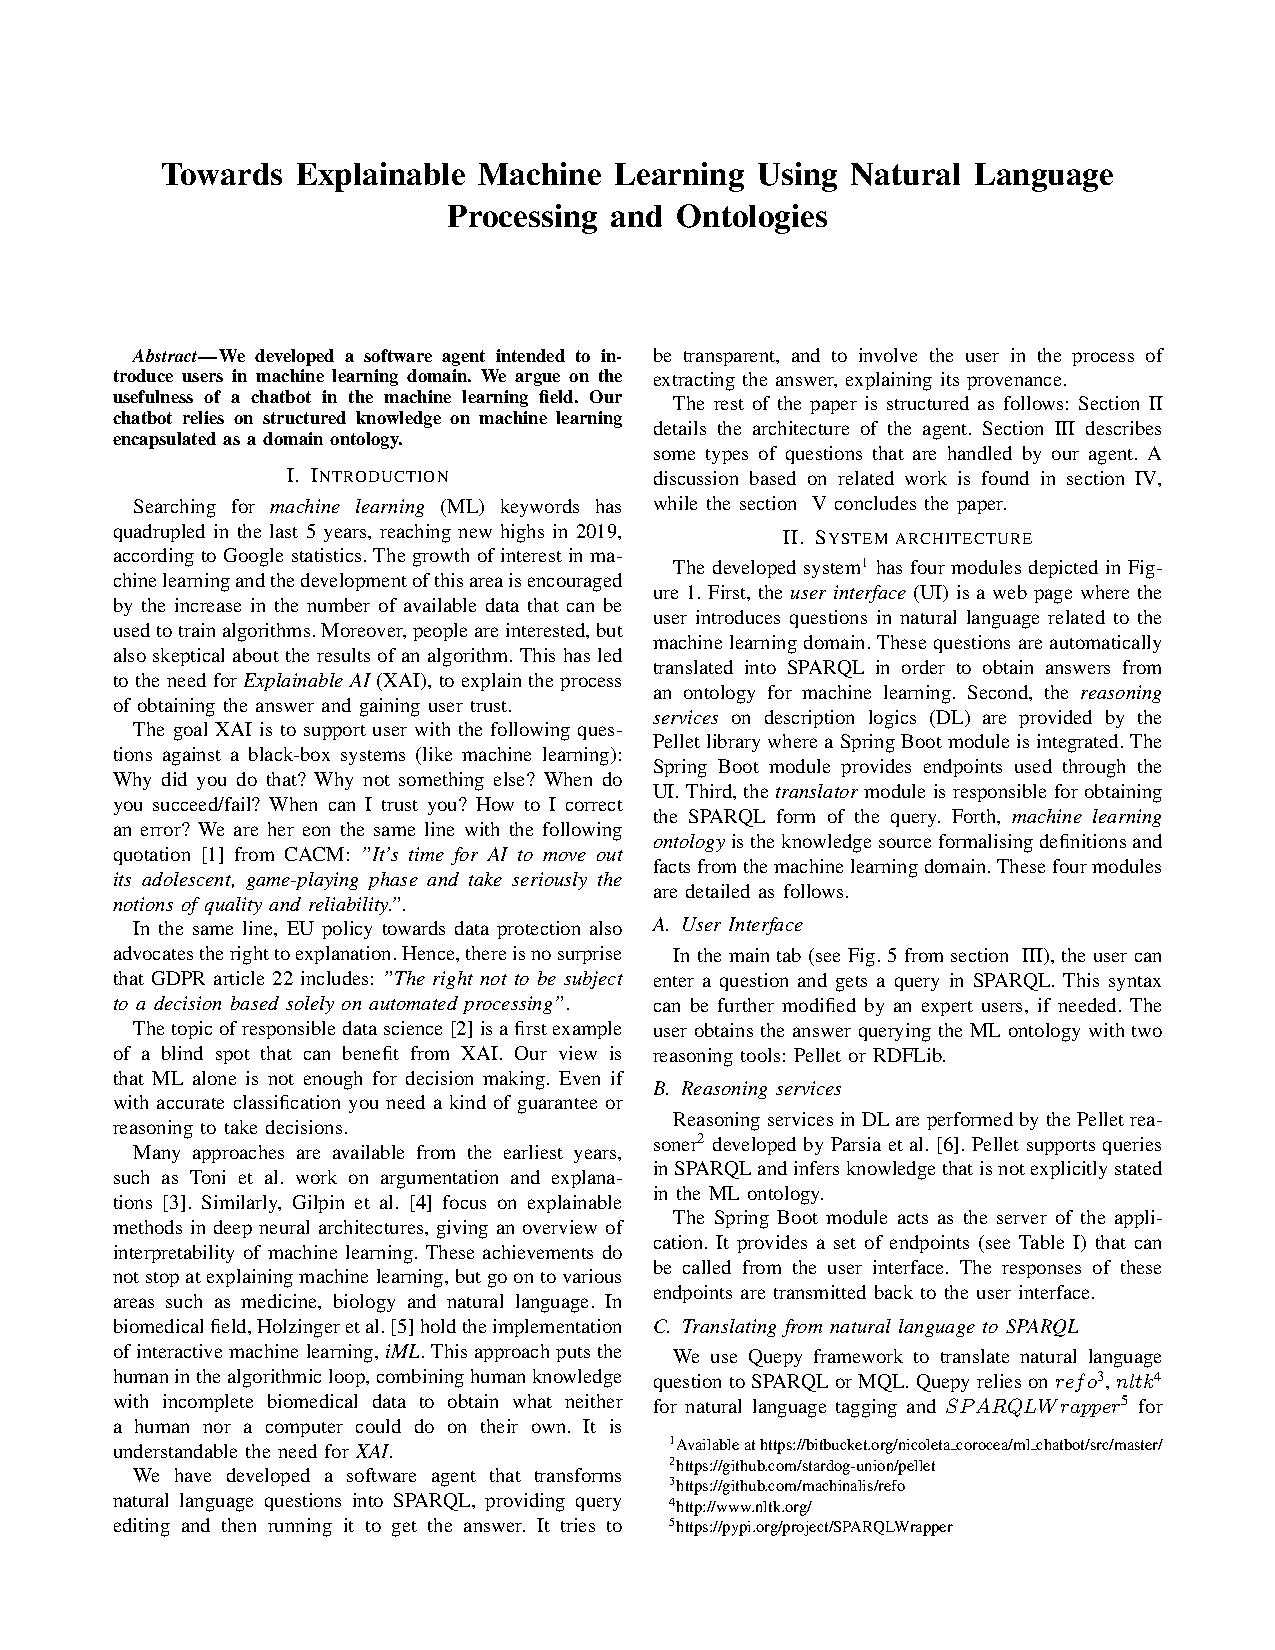
\includepdf[pages=-,pagecommand={},width=\textwidth]{articol_extins.pdf}
